

\newpage

\section{Anexos}

\subsection{Declaración de Uso de Herramientas de Inteligencia Artificial}
\label{sec:declaracion_ia}

Durante el proceso de redacción y preparación del presente documento de grado, se utilizó el modelo de inteligencia artificial \textbf{ChatGPT (versión de julio de 2024)} \cite{chatgpt} como herramienta de apoyo tecnológico. 

El uso de esta herramienta se limitó estrictamente a:
\begin{itemize}
    \item Corrección gramatical y ortográfica.
    \item Sugerencias de fluidez y estilo de redacción.
\end{itemize}

Cabe destacar que la formulación del problema, la investigación técnica, el desarrollo metodológico, el análisis de los resultados y las conclusiones son de autoría exclusiva del autor del documento, no habiéndose delegado en la inteligencia artificial la generación de contenido intelectual o técnico.

\subsection{Imágenes}
\begin{figure}[H]
    \centering
    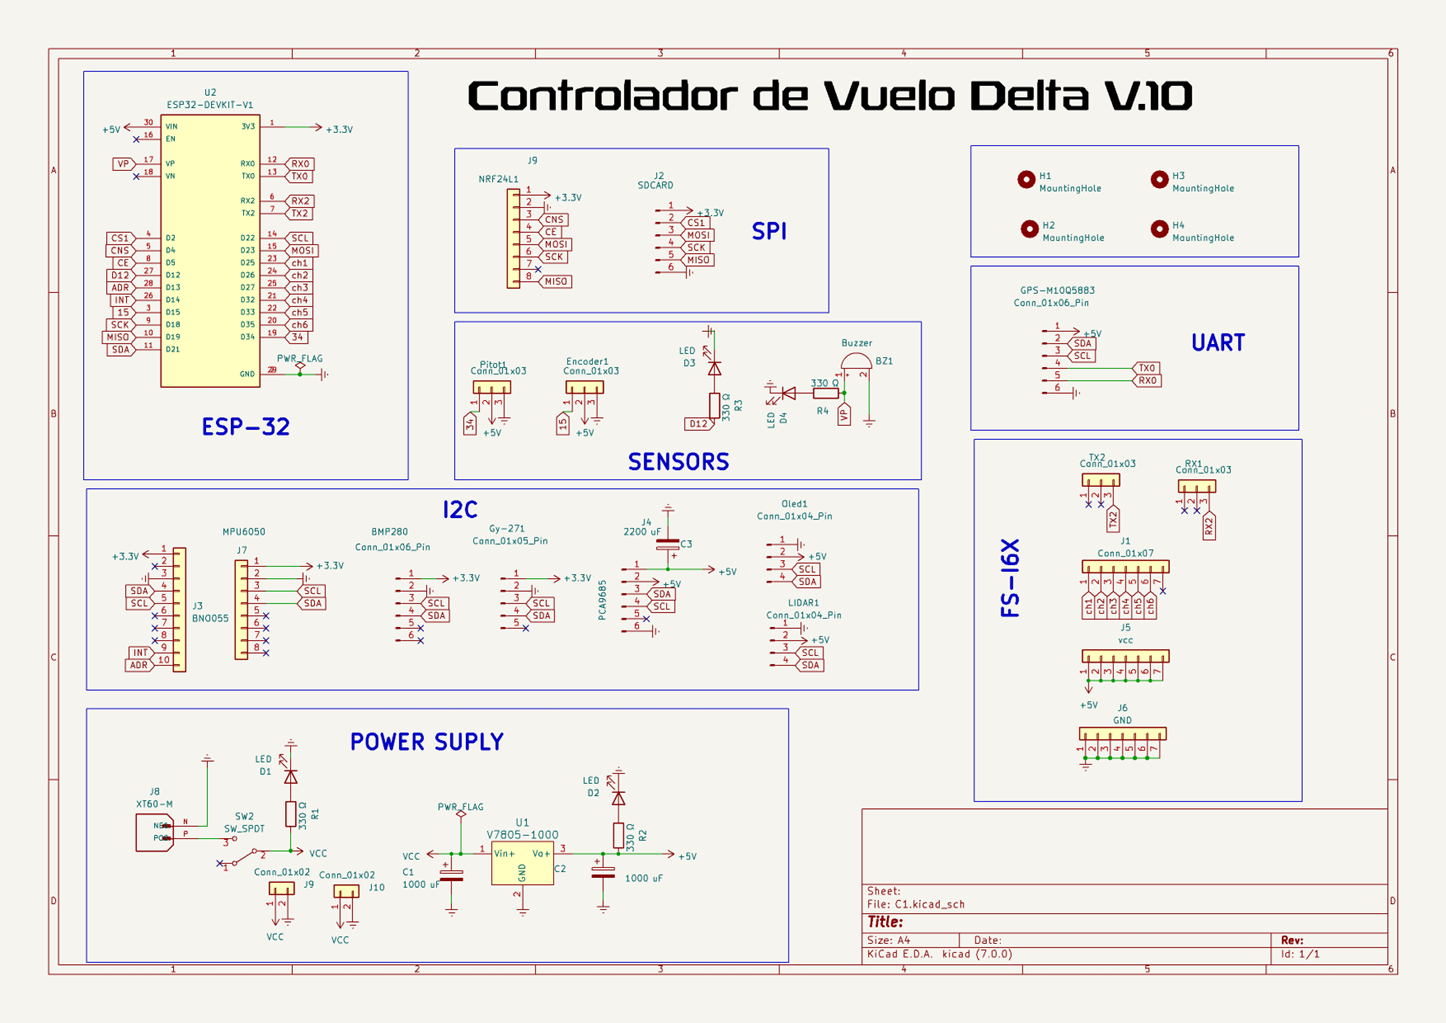
\includegraphics[width=\textwidth]{Imagenes/Anexos/esquematico_controlador_v1.png}
    \caption{Esquemático Circuito Impreso 1.0 }
    \label{fig:sch-1.0}
\end{figure}

\begin{figure}[H]
    \centering
    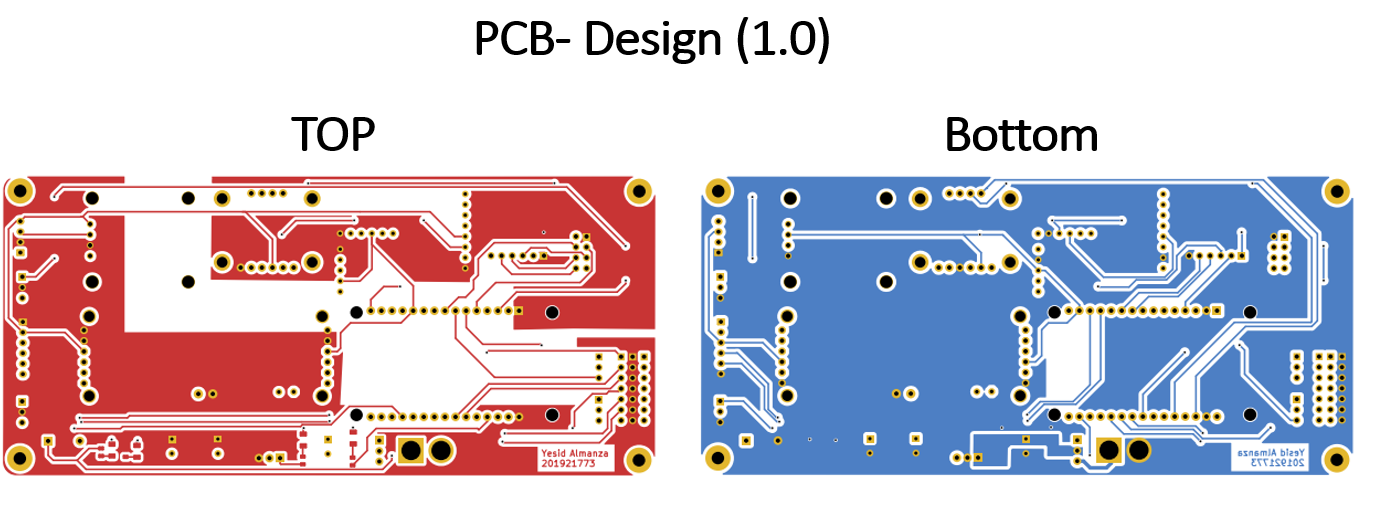
\includegraphics[width=\textwidth]{Imagenes/Anexos/layout_pcb.png}
    \caption{Layout Circuito Impreso 1.0 }
    \label{fig:pcb-1.0}
\end{figure}

\begin{figure}[H]
    \centering
    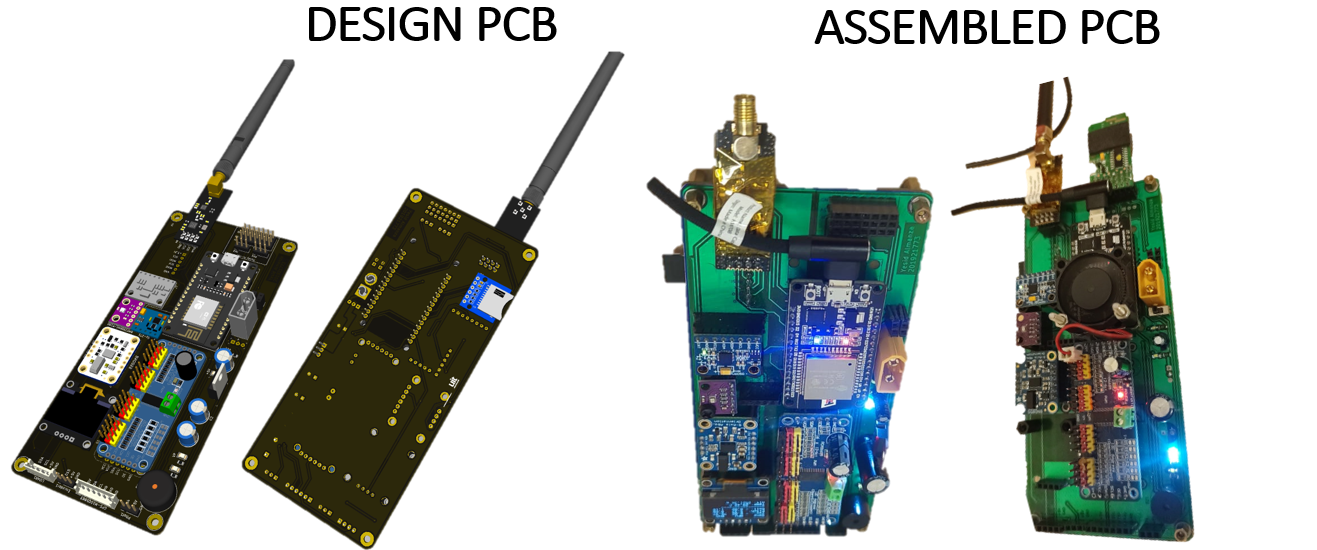
\includegraphics[width=\textwidth]{Imagenes/Anexos/pcb_primera_iteracion.png}
    \caption{Circuito Impreso Ensamblado 1.0 }
    \label{fig:pcb-ensambled-1.0}
\end{figure}

\begin{figure}[H]
    \centering
    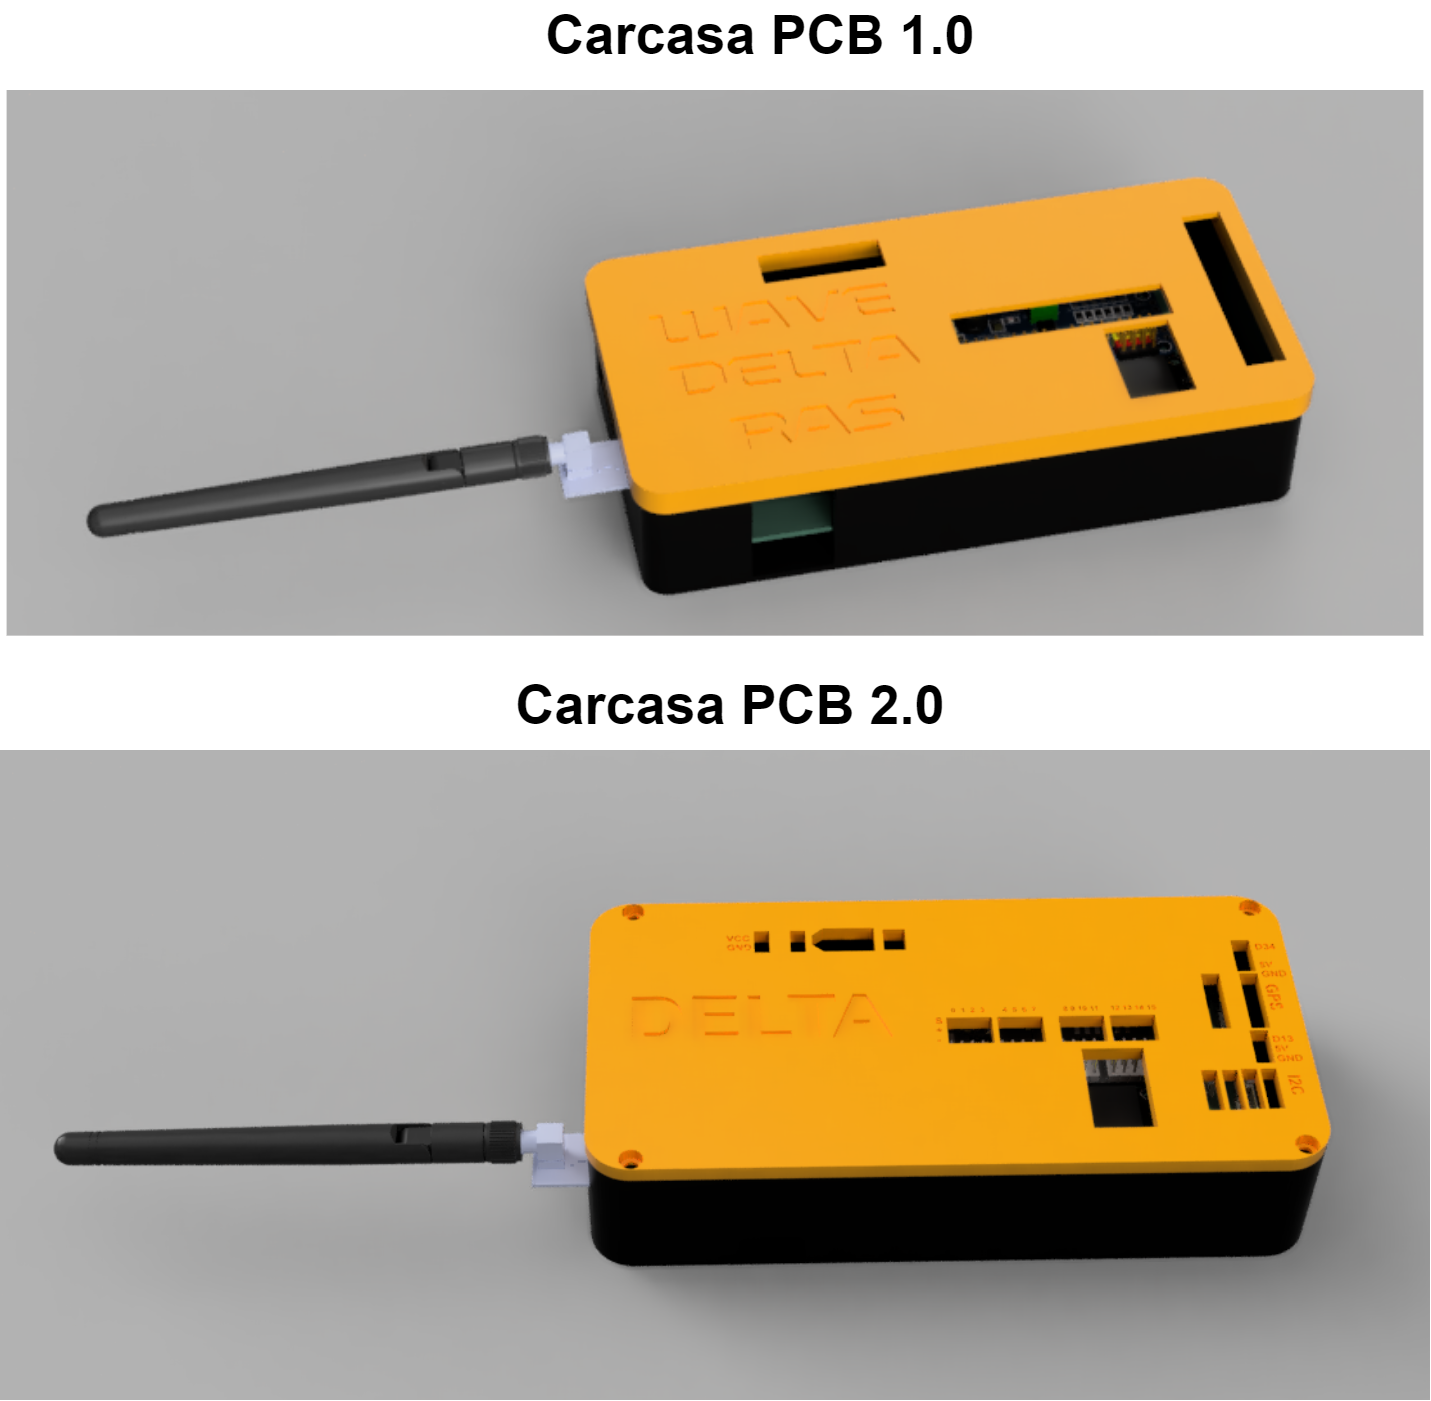
\includegraphics[width=\textwidth]{Imagenes/Anexos/carcasa_version.png}
    \caption{Carcasas Versiones }
    \label{fig:carcasasVersion}
\end{figure}

